\documentclass[11pt]{article}
\usepackage[T1]{fontenc}
\usepackage{lmodern,microtype}
\usepackage[a4paper,margin=26mm]{geometry}
\usepackage{amsmath,amssymb,amsthm,mathtools,bm}
\usepackage{graphicx,booktabs,array,enumitem,longtable}
\usepackage[numbers,sort&compress]{natbib}
\usepackage{xcolor}
\usepackage[colorlinks=true,linkcolor=blue!50!black,citecolor=blue!50!black,urlcolor=blue!50!black]{hyperref}
\usepackage{xurl}
\newtheorem{theorem}{Theorem}[section]
\newtheorem{proposition}[theorem]{Proposition}
\newtheorem{lemma}[theorem]{Lemma}
\theoremstyle{remark}\newtheorem{remark}[theorem]{Remark}
\newcommand{\E}{\mathbb E}
\newcommand{\KL}{D_{\rm KL}}
\graphicspath{{../figures/}}
\setcounter{tocdepth}{1}
\hypersetup{pdftitle={From Represented Information to Realizable Neural Growth},pdfauthor={Wenyu Huang}}
\title{From Represented Information to Realizable Neural Growth\\[5pt]
\large Observation Limits, Singular Positive Splits, and Finite-Sample Tests}
\author{Wenyu Huang\\University of California San Diego}
\date{Phase II companion research manuscript \;|\; September 13, 2026}
\begin{document}
\maketitle
\begin{abstract}
Can information about a learning unit guide its structural adaptation?
We distinguish information retained by a representation, information observed
by a controller, and improvement accessible to a specified neural operation.
An explicit full-support four-input tanh classifier is a population local
minimum while retaining no task information. Two tasks have identical
activation--label--residual laws but require different split directions:
no passive controller restricted to that law can select an immediate split
with positive expected loss reduction on both tasks, even with unlimited
samples. Input--residual context permits strict descent, with
matching sample order in a two-task identification problem. A separate
noisy-parity construction has positive task information and zero splitting
matrix. At the same two-child width and positive normalized output weights,
fixed-proportion centered splits increase log loss at order $t^4$, whereas
a child proportion of order $t^{d-4}$ yields a strictly decreasing path at
order $t^{2d-4}$. This is a constrained nonuniform-limit calculation; curvature
splitting, parity blindness, and boundary-weight escape have prior precedents.
Actual finite-sample tanh training tests the observation bridge against
random growth, continued training, fixed-width models, and an explicitly
privileged oracle. Geometry helps at a designed initial state under short
training budgets; that benefit erodes with longer training and altered
initialization. Information-score experiments and holdout gates expose
additional estimation and optimization failures. The results establish
specific limits and a restricted trainable bridge, not a universal
information-driven growth algorithm.
\end{abstract}
\tableofcontents

\section{The scientific question after Phase I}
The motivating question is whether a learning system can use what its units
represent or process to decide autonomously how its structure should change.
Activation entropy and neuron splitting are candidate ingredients, not
scientific commitments. A useful answer must identify both the information
available to the controller and the operations its learning system can perform.

The preserved Phase I manuscript, \emph{The Price of Irreversible
Representation Growth: Sharp Four-State Obstructions under Logarithmic Loss},
studies a different object: finite encoders under hard alphabet budgets.
It proves a sharp obstruction to simultaneously competitive nested encoders.
Its four-state construction and reassignment calculation do not identify
states with neurons or bound neural optimization cost. We use its warning
about restricted operations as a diagnostic, and move to explicit neural
parameters. The new theory does not depend on the unreviewed information-
bottleneck onset draft preserved with that project.

The central advance is a pair of inspectable separations and their learning
tests. First, a summary can be perfectly estimated yet omit the pairing
between residuals and inputs that selects a useful operation. Second, even
with that pairing known, structural accessibility depends on the way output
weights and incoming perturbations approach a growth event. These claims are
more specific than saying that entropy is insufficient. They give an exact
observation model, strict population descent alternatives, and failure tests
for an actual parameterized learner.

We intentionally separate three questions. Does a representation contain
information predictive of the target? Can a controller distinguish which
structural operation helps from its observations? Does the allowed operation,
followed by the implemented optimizer and data budget, realize the benefit?
The experiments do not promote a positive answer to one question into a
positive answer to the others.

\subsection{What was explored and why this direction was selected}
Independent investigations began with the broad original question. They
considered finite-state reassignment, information-bottleneck birth geometry,
conditional-information operation selection, neural splitting, and local
observational limitations. Extending the Phase I source-mass rate remained
mathematically interesting but would retain the same rare-state population
abstraction. An exact conditional-information rule for Bayes-refitted cells
would have a direct decision-tree interpretation and insufficient neural
content. Re-deriving negative-curvature growth would duplicate established
methods. The chosen route instead exposes a missing premise in transferring
information criteria to neural operations, and supplies actual tests of the
most direct existing geometric remedy.

The observation example would be undermined by a controller identifying both
tasks using only the stipulated identical observation laws. The high-order
result would be undermined by a negative fixed-proportion small-radius path
under its stated restrictions or a failure of the joint-limit coefficient.
The empirical hypothesis that task-information scores select useful neural
operations is undermined when equal-size, equal-training comparisons favor
random or fixed-width alternatives. Those counterexamples and negative
comparisons were actively retained.

\section{Starting-point audit and evidence types}
\label{sec:audit}
All supplied Phase I sources, results, and the authoritative PDF were
preserved before modifications in a 63-file ZIP snapshot with per-file
SHA-256 hashes. The original project has no supplied Git revision; the
hash manifest is the starting identifier. Original-code evaluations at
$L=16,64,256,2048$ match eight stored quantities at all 60 saved digits.
An independent implementation enumerates function tables and computes risk
from joint probabilities rather than using the original partition recursion
and entropy-difference routine. It recovers 15 partitions and 18 compatible
chains; nine compared quantities agree to relative tolerance $10^{-58}$.
The deterministic total-risk prices are respectively $2.191327$, $4.641185$,
$9.499428$, and $27.125385$. The audited core proofs revealed no substantive
mathematical error. This is an audit of the claims used here, not a new
formal certification of every Phase I result.

There are three distinct kinds of Phase II evidence. Theorems below are
population statements with full proofs. Exhaustive population calculations
check finite neural operations and asymptotic coefficients. Finite-sample
experiments fit neural parameters or estimate controller statistics from
sampled labels; the evaluator may integrate against the known synthetic law,
but those population probabilities are withheld from implemented controllers.
Using such an evaluator does not convert finite-sample fitting into oracle
learning. Likewise the high-order construction is an oracle existence path,
not a trained adaptive mechanism.

\section{Nearest results and the bounded novelty claim}
\label{sec:related}
Splitting steepest descent already derives a residual-weighted neural
splitting matrix and negative-eigenvalue binary growth
\cite[Sections 2.1--2.3, Theorems 2.2--2.4]{ssd2019}. Signed splitting
optimizes the analogous second-order form with signed normalized coefficients
\cite[Theorems 2.1--2.3]{signed2021}; Firefly studies broader function-space
growth neighborhoods and optimized candidate additions
\cite[Sections 2.1--2.3]{firefly2020}. The controller used in our curvature
experiment is an explicit implementation of the established splitting
principle. It is not a new entropy-based algorithm.

The closest boundary result is Ding, Li, and Sun's stationary-plateau
analysis \cite{ding2026}. Their Theorem 3 and its proof in Section 6.3.1
cover locally effective neurons with zero inner Hessian under square loss,
using a dormant child's small outgoing coefficient and nearby input weight.
Thus neither higher-order effectiveness nor escape through zero output
weight is first established here. Our additional calculation enforces
strictly positive normalized weights at every nonzero radius, two children,
an exactly conserved weighted incoming mean, and logistic loss; it identifies
the explicit parity-dependent weight and risk orders, against an
interior-proportion obstruction. We found no equivalent statement with this
combination in the inspected sources, but do not claim an exhaustive
historical search.

The need to specify local observations and feedback has long been emphasized
in local-learning theory \cite[Sections 6.4 and 7.1]{baldi2016}.
Information-theoretic neuron learning also has concrete precedents:
infomorphic networks use richer presynaptic and context signals
\cite{makkeh2025}. Our activation-summary restriction excludes that richer
input access. It is not an impossibility of local synaptic learning or a
claim of the first information-theoretic neural implementation.

Parity orthogonality and gradient blindness are established themes
\cite[Section 2]{failures2017}. More recent work proves hardness for fixed
parities in specific ReLU/perturbed-gradient settings \cite{shoshani2025},
while learnability can change under specially structured distributions
\cite{daniely2020}. Our fixed-dimension Taylor calculation does not claim
new general parity hardness. The moment identities, testing inequalities,
and log-loss identities in the proofs are standard tools; the contribution
is their exact constrained neural witnesses and the accompanying evidence.
A source-by-source record, versions, inspected locations, and unresolved
novelty risks are supplied in \texttt{research/prior\_art.md}.

% Complete Phase II proofs. Parent manuscript supplies theorem environments.
\section{What an activation-only controller cannot observe}
\label{sec:activation-observation}

We now study actual neural parameters. This model has no discrete
representation-cardinality constraint. Its purpose is to separate an
information summary from the information needed to realize a structural
operation. The observation restriction below is explicit: a physical unit
may also have access to presynaptic inputs, in which case the negative
result does not apply.

Let $X$ be uniform on $\{e_1,-e_1,e_2,-e_2\}\subset\mathbb R^2$.
For an unknown task $s\in\{-1,+1\}$ and $0<\eta<1/2$, set
\[
 q_s(\pm e_1)=\mathbb P_s(Y=1\mid X=\pm e_1)=\tfrac12+s\eta,
 \qquad q_s(\pm e_2)=\tfrac12-s\eta.
\]
Every source-label pair has positive probability. Write
$\phi(t)=\tanh t$ and use binary log loss
$\ell(f,y)=\log(1+e^f)-yf$. A one-hidden-unit network has logit
$f(x)=c+a\phi(b+w^\top x)$. Fix $b=b_0>0$, $a=1$, $w=0$, and
$c=-\phi(b_0)$, so that $f_0=0$ and the predicted probability is $1/2$.
At this point the activation is $A=\phi(b_0)$ and the output residual is
$R=1/2-Y$. All logs below are natural.

\begin{proposition}[A parameter local minimum with unrepresented task information]
\label{prop:axis-local-min}
If
\begin{equation}
 0<\eta<\frac{\phi'(b_0)^2}{4|\phi''(b_0)|},
 \label{eq:axis-stability}
\end{equation}
the stated one-unit parameter vector is a local minimum of population
log loss on either task. It lies on a manifold of equivalent constant
predictors. Nevertheless
\[
 I_s(X;Y)=\log2-h(\tfrac12+\eta)>0,
 \qquad I_s(A;Y)=0.
\]
The entire laws of $(A,Y,R)$ are identical for the two tasks.
\end{proposition}
\begin{proof}
Introduce the smooth invertible coordinate $r=c+a\phi(b)$, retaining
$a,b,w$. Then
$f(x)=r+a\{\phi(b+w^\top x)-\phi(b)\}$.
For every $a,b$ near $1,b_0$, the risk as a function of $(r,w)$ is
stationary at $(0,0)$: its $r$ derivative is
$\mathbb E_s(1/2-Y)=0$, and its $w$ derivative is
$a\phi'(b)\mathbb E_s[(1/2-Y)X]=0$ by sign symmetry of each axis.
At this point its Hessian in the $(r,w)$ coordinates is block diagonal,
with $rr$ entry $1/4$ and $ww$ block
\begin{equation}
 \frac{a^2\phi'(b)^2}{8}I_2
 +a\phi''(b)
 \begin{pmatrix}-s\eta/2&0\\0&s\eta/2\end{pmatrix}.
 \label{eq:axis-hessian}
\end{equation}
Indeed $\ell_f=1/2-Y$, $\ell_{ff}=1/4$ at zero,
$\mathbb E XX^\top=I_2/2$, and the mixed $rw$ entries vanish because
$\mathbb EX=0$. Under \eqref{eq:axis-stability} this Hessian is
positive definite at $(a,b)=(1,b_0)$. By continuity there is a compact
neighborhood of $(1,b_0,0,0)$ and $m>0$ on which the $(r,w)$ Hessian is
bounded below by $mI_3$. Taylor's integral formula along the line from
$(0,0)$ to $(r,w)$, with $a,b$ fixed, therefore gives
\[
 L_s(r,w;a,b)-\log2\ge \frac m2(r^2+\|w\|^2)
\]
throughout a smaller neighborhood. At $r=w=0$ the risk remains $\log2$
for all nearby $a,b$. This proves a local minimum in all original
parameters, allowing its neutral directions.

The marginal law of $Y$ is Bernoulli$(1/2)$ and every input has
conditional entropy $h(1/2+\eta)$; the information formula follows.
Since $A$ is constant, and $R$ is a function of $Y$, the final assertions
follow as well.
\end{proof}

Replace the hidden unit by two units of output weight $1/2$, biases
$b_0$, and incoming weights $+\epsilon v,-\epsilon v$, retaining the
intercept $-\phi(b_0)$, where $\|v\|=1$. The resulting logit is
\begin{equation}
 f_{\epsilon,v}(x)=\frac{\phi(b_0+\epsilon v^\top x)
 +\phi(b_0-\epsilon v^\top x)}2-\phi(b_0).
 \label{eq:axis-split}
\end{equation}
At $\epsilon=0$ this is a function-preserving duplication; at positive
$\epsilon$ it is the specified structural perturbation. This familiar
symmetric split is the operation studied in splitting steepest descent;
the score derived below is not claimed as new.

For $t\ge0$ put
\begin{equation}
 d(t)=\phi(b_0)-\frac{\phi(b_0+t)+\phi(b_0-t)}2
 =\frac{z(1-z^2)\tanh^2t}{1-z^2\tanh^2t},\qquad z=\tanh b_0.
 \label{eq:axis-d}
\end{equation}
Thus $d(0)=0$ and $0<d(t)<z$ for $t>0$.

\begin{theorem}[Exact observation-channel obstruction and attainable descent]
\label{thm:axis-observation}
Let $\Delta_s(\epsilon,v)=L_s(f_{\epsilon,v})-\log2$, and put
$d_j=d(|\epsilon v_j|)$. Then
\begin{equation}
 \Delta_s(\epsilon,v)
 =\frac12\left\{\log\cosh(d_1/2)+\log\cosh(d_2/2)\right\}
   +\frac{s\eta}{2}(d_1-d_2).
 \label{eq:axis-risk}
\end{equation}
Consequently:
\begin{enumerate}
\item Any possibly randomized controller whose entire task-dependent
observation consists of the population law of $(A,Y,R)$, or any number
of independent samples from that law, satisfies
\[
 \max_{s\in\{-1,+1\}}\mathbb E_s
       \Delta_s(\epsilon,v)\ge0.
\]
Here it may select both $\epsilon\ge0$ and the unit vector $v$ from
these observations. Expectations include its observations and randomness;
risk is evaluated on a fresh population input. The controller may also
decline to split, which gives zero change.
\item A controller with the input-residual second moment
$M_s=\mathbb E_s[(1/2-Y)XX^\top]$ can choose $v=e_2$ for $s=+1$
and $v=e_1$ for $s=-1$. For either task its exact gain is
\begin{equation}
 G(\epsilon,\eta)
 =\frac{\eta d(\epsilon)}2
  -\frac12\log\cosh\{d(\epsilon)/2\}
 \ge\frac{\eta d(\epsilon)}2-\frac{d(\epsilon)^2}{16}>0
 \label{eq:axis-gain}
\end{equation}
whenever $0<d(\epsilon)<8\eta$.
\end{enumerate}
\end{theorem}
\begin{proof}
The addition formulas for $\tanh(b_0\pm t)$ give
\eqref{eq:axis-d}; its denominator is positive. At either point on
axis $j$, the split logit is $-d_j$. For any posterior $q$,
\[
 \mathbb E[\ell(-d,Y)\mid q]-\log2
 =\log\cosh(d/2)+(q-1/2)d.
\]
Averaging the two axes proves \eqref{eq:axis-risk}.

The two tasks give identical laws of all permitted controller
observations. Consequently its joint distribution of $(\epsilon,v)$
is the same under both tasks, including when selected from a random
sample. Pointwise,
\[
 \Delta_+(\epsilon,v)+\Delta_-(\epsilon,v)
 =\log\cosh(d_1/2)+\log\cosh(d_2/2)\ge0.
\]
Taking the common expectation proves the first part. Independent
controller randomization cannot change this calculation.

The matrix is $M_s=\operatorname{diag}(-s\eta/2,s\eta/2)$, so it
identifies the displayed axis choice. Substituting it in
\eqref{eq:axis-risk} gives the gain. To verify the inequality used
in \eqref{eq:axis-gain}, for $u\ge0$ one has $\tanh u\le u$, because
the derivative of $u-\tanh u$ is $\tanh^2u\ge0$ and the value at zero
is zero. Integrating gives $\log\cosh u\le u^2/2$; evenness handles
$u<0$. The strict positivity follows from $d<8\eta$.
\end{proof}

For orientation, Taylor expansion of \eqref{eq:axis-split} yields
\[
 \Delta_s(\epsilon,v)
 =\frac{\epsilon^2}{2}v^\top S_s v+O(\epsilon^4),
 \qquad S_s=\phi''(b_0)M_s.
\]
This is the established splitting matrix specialized to log loss.
Theorem~\ref{thm:axis-observation} adds an exact finite-displacement
statement about which observation channels can select its useful
direction. It does not require naming $M_s$ an entropy estimator or a
unique-information decomposition. In particular, even the scalar
$I_s(X;Y)$ is identical across the tasks and does not specify an axis.

\begin{theorem}[Finite observations: sufficient and necessary sample order]
\label{thm:axis-samples}
Suppose the controller receives $n$ independent full pairs $(X_i,Y_i)$.
Define
\[
 U_i=(1/2-Y_i)(X_{i2}^2-X_{i1}^2),\qquad
 \widehat s=\operatorname{sign}\Big(\sum_{i=1}^n U_i\Big),
\]
with any fixed rule for a zero sum. Select the axis prescribed in
Theorem~\ref{thm:axis-observation} for $\widehat s$, with fixed
$\epsilon>0$ satisfying $d(\epsilon)<8\eta$. On either task,
\begin{equation}
 \mathbb P_s\{\Delta_s=-G(\epsilon,\eta)\}
 \ge1-\exp(-2n\eta^2).
 \label{eq:axis-sample-upper}
\end{equation}
Conversely, for any randomized procedure selecting a symmetric split
from $n$ full observations, if its probability of strict population
descent is at least $1-\delta$ on each task, where $0<\delta<1/4$,
then
\begin{equation}
 n\ge\frac{\log(1/(4\delta))}{-\log(1-4\eta^2)}.
 \label{eq:axis-sample-lower}
\end{equation}
For $0<\eta\le1/4$, the right hand side is at least
$3\log(1/(4\delta))/(16\eta^2)$.
\end{theorem}
\begin{proof}
For task $s$, $U_i$ takes values $\pm1/2$ and has mean $s\eta$.
Hoeffding's inequality for independent variables with range length one
therefore gives
$\mathbb P_s(s\sum_i U_i\le0)\le e^{-2n\eta^2}$.
For completeness its exponential bound follows by applying Markov's
inequality to $e^{-t\sum_i(sU_i-\eta)}$, using the bounded-variable
moment generating function inequality
$\mathbb Ee^{t(V-\mathbb EV)}\le e^{t^2/8}$ for an interval of length
one, and minimizing $e^{-tn\eta+nt^2/8}$ at $t=4\eta$.
The moment generating function inequality follows from convexity by
bounding $e^{tV}$ by its endpoint chord and maximizing the centered
two-point expression (or by twice integrating that expression's
second logarithmic derivative, which is a Bernoulli variance at most
$1/4$). Correct identification gives exactly the claimed gain.

Any selected split with $\Delta_s<0$ must, by \eqref{eq:axis-risk},
satisfy $s(d_2-d_1)>0$. Therefore a procedure that achieves strict
descent with probability at least $1-\delta$ yields a test for $s$
with each error probability at most $\delta$: report $+1$ when
$d_2>d_1$ and $-1$ otherwise. Extra independent randomization cannot
improve the optimal testing error.

Write $P_+,P_-$ for the two laws of a full pair. Their Hellinger
affinity is
\[
 \rho=\sum_{x,y}\sqrt{P_+(x,y)P_-(x,y)}
     =\sqrt{1-4\eta^2}.
\]
The affinity of product laws is $\rho^n$. For arbitrary finite laws
$P,Q$ with affinity $a$, Cauchy--Schwarz gives
\[
 \|P-Q\|_{\rm TV}
 =\frac12\sum_z|\sqrt{P(z)}-\sqrt{Q(z)}|
                 (\sqrt{P(z)}+\sqrt{Q(z)})
 \le\sqrt{1-a^2}.
\]
The sum of type-I and type-II errors of any test is at least
$1-\|P-Q\|_{\rm TV}$: this follows directly by writing its acceptance
probability as a function in $[0,1]$ and bounding the difference of
expectations by total variation. Its equal-prior average error is
thus at least
\[
 \frac{1-\sqrt{1-\rho^{2n}}}{2}\ge\frac{\rho^{2n}}4
 =\frac{(1-4\eta^2)^n}4,
\]
where the inequality uses $1-\sqrt{1-t}=t/(1+\sqrt{1-t})\ge t/2$.
Both errors at most $\delta$ imply \eqref{eq:axis-sample-lower}.
Finally $-\log(1-u)=\int_0^u(1-t)^{-1}dt\le u/(1-u)$ and
$u=4\eta^2\le1/4$ imply
$-\log(1-4\eta^2)\le16\eta^2/3$.
\end{proof}

The lower bound applies even to a controller given full inputs; the
activation-only controller receives no task-identifying information at
any sample size. The upper bound uses ordinary independent sampling,
not an oracle population covariance. Neither statement predicts the
outcome of unrestricted training after the operation. Such training
observes input coordinates and can learn distinctions unavailable to
the restricted structural controller.


\section{Equal width, unequal access: a nonuniform positive split limit}
\label{sec:highorder}
The preceding example concerns missing observations. Even full population
information does not make a fixed structural operation effective. We now
hold the number of children, positivity and sum of outgoing weights, and
weighted incoming mean fixed, but change the relation between the child
weight and the size of the incoming perturbation. This is a restricted
separation, not a new discovery of parity hardness or boundary-weight
escape; see Section~\ref{sec:related}.

Let $d\ge6$ be even, $X$ uniform on $\{-1,1\}^d$, and
$\chi(X)=\prod_{j=1}^d X_j$. For $0<\eta<1/2$, set
\begin{equation}\label{eq:paritylaw}
 \Pr(Y=1\mid X=x)=\tfrac12+\eta\chi(x).
\end{equation}
This law has full support and $I(X;Y)=\log2-h(1/2+\eta)>0$,
independently of $d$. No limiting rare source mass is used when $d$ is fixed.
Fix a smooth activation $\sigma$ near $b$ with
$\sigma''(b)\ne0$ and $\sigma^{(d)}(b)\ne0$, with bounded derivatives
through order $d+2$ there. The experiments use $\sigma=\tanh$ and $b=1/2$.
The parent logit is the constant $\sigma(b)-\sigma(b)=0$.
For a unit vector $v$ put $V=v^\top X$, and define a positive binary split
\begin{equation}\label{eq:asymmetric}
 f_{t,p}(x)=p\sigma(b+tV)+(1-p)\sigma\left(b-\frac{p}{1-p}tV\right)-\sigma(b),
 \quad 0<p<1.
\end{equation}
There are exactly two hidden units. Their outgoing weights sum to one,
their weighted incoming mean is zero, and their outgoing $\ell_1$ norm is
one. For $p\le1/2$, both incoming weights have norm at most $t$.
The intercept stays fixed in this comparison; we do not claim an obstruction
after arbitrary intercept refitting or subsequent parameter training.

Write $R(f)=\E[\log(1+e^{f(X)})-Yf(X)]$ and
\begin{equation}\label{eq:KB}
 K(v)=\frac{\sigma''(b)^2}{32}\E V^4>0,
 \qquad B(v)=\sigma^{(d)}(b)\prod_{j=1}^d v_j.
\end{equation}
A direction with $B(v)>0$ exists by changing the sign of one nonzero
coordinate. Its selection here is an oracle construction.

\begin{theorem}[A constrained weight--radius separation]\label{thm:boundary}
Under the preceding conditions:
\begin{enumerate}[label=(\roman*)]
\item For every fixed $p\in(0,1)$ and unit $v$,
\[
 R(f_{t,p})-\log2
   =K(v)\left(\frac{p}{1-p}\right)^2t^4+o(t^4)>0
\]
for all sufficiently small positive $t$. This positivity is uniform when
$p$ lies in any compact subinterval of $(0,1)$ and $v$ ranges over the unit sphere.
\item Choose $B(v)>0$ and let $p(t)=\kappa t^{d-4}$ for fixed $\kappa>0$.
Then
\begin{equation}\label{eq:jointlimit}
 R(f_{t,p(t)})-\log2
 =\{K(v)\kappa^2-\eta B(v)\kappa\}t^{2d-4}
    +o(t^{2d-4}).
\end{equation}
In particular, the choice
\[\kappa=\frac{\eta B(v)}{2K(v)}\]
gives strict descent with leading coefficient
\[ -\frac{\eta^2B(v)^2}{4K(v)}.\]
\item At the constant parent, the residual splitting matrix is zero.
More generally the derivatives in incoming weights of the label-dependent
part of the population loss agree with the independent-label law through
every order strictly below $d$.
\end{enumerate}
\end{theorem}

\begin{proof}
For every integer $j<d$, $\E[\chi(X)V^j]=0$. Indeed expand $V^j$
into monomials: at least one coordinate has even exponent (possibly zero),
and multiplication by $\chi$ makes its expectation zero. At degree $d$,
the only surviving monomials use each coordinate once, so
\begin{equation}\label{eq:fouriermoment}
 \E[\chi V^d]=d!\prod_i v_i.
\end{equation}
Odd-degree moments with $\chi$ vanish here because $d$ is even and the law
is invariant under $X\mapsto-X$.
The exact loss identity is
\begin{equation}\label{eq:parityrisk}
 R(f)-\log2=\E\log\cosh(f/2)-\eta\E[\chi f].
\end{equation}
For fixed $p$, Taylor expansion of \eqref{eq:asymmetric} cancels the constant
and linear terms and gives, uniformly on the finite input set,
\[
 f_{t,p}=\frac{\sigma''(b)}2\frac{p}{1-p}t^2 V^2+O(t^3).
\]
Since $\log\cosh(z/2)=z^2/8+O(z^4)$, its convexity penalty has leading
term $K(v)[p/(1-p)]^2t^4$. Equations~\eqref{eq:fouriermoment}
and the Taylor expansion through order $d$ show that $\E[\chi f_{t,p}]=O(t^d)$.
Thus the signal is $o(t^4)$. Uniformity on compact $p$ intervals follows
from bounded derivatives and $|V|\le\sqrt d$; $\E V^4\ge(\E V^2)^2=1$
ensures a uniform positive leading coefficient.

For the joint limit it is important to retain the factor $p$ in the
remainders. Put $q=p/(1-p)$. For $p\le1/2$, the two Taylor remainders of
order three are bounded by $C[p+(1-p)q^3]t^3=O(pt^3)$.
Consequently, as both $p,t\to0$,
\[
 f_{t,p}=\tfrac12\sigma''(b)\,p t^2 V^2\{1+O(p)\}+O(pt^3),
\]
where the braces apply to the displayed leading term, not to a pointwise
relative error at $V=0$. It follows that
\begin{equation}\label{eq:penaltyjoint}
 \E\log\cosh(f_{t,p}/2)=K(v)p^2t^4\{1+O(p)+O(t)\}.
\end{equation}
Expanding through order $d+1$, all lower-degree terms and the degree-$d+1$
term disappear after multiplying by $\chi$. The remaining Taylor errors
are $O(pt^{d+2})$. Hence
\begin{align*}
 \E[\chi f_{t,p}]
 &=B(v)t^d\left\{p+(1-p)\left(\frac p{1-p}\right)^d\right\}
    +O(pt^{d+2})\\
 &=B(v)pt^d\{1+O(p^{d-1})+O(t^2)\},
\end{align*}
where the last line uses $B(v)>0$ fixed. Substitute
$p=\kappa t^{d-4}$ into this formula and \eqref{eq:penaltyjoint}.
Both leading terms then have order $t^{2d-4}$, proving
\eqref{eq:jointlimit}. The optimizing coefficient is obtained by completing
the square; $p(t)\in(0,1/2]$ eventually.

Finally, the residual splitting matrix is
$-\eta\sigma''(b)\E[\chi XX^\top]=0$ by the same moment argument.
The difference of the parity-task risk and the independent-label risk for
any logit $f$ is exactly $-\eta\E[\chi f]$. For a finite sum of smooth
neurons with zero incoming weights, any derivative of this difference in
incoming coordinates of total order less than $d$ is a linear combination
of moments $\E[\chi X^\alpha]$ with $|\alpha|<d$, and vanishes. This proves
(iii). It asserts a derivative identity, not an impossibility for arbitrary
sample-based algorithms, active probing, or optimization away from the parent.
\end{proof}

The decreasing path approaches an embedding with a zero-output child at
$t=0$. It is not a small perturbation of the equal-weight duplication in
the full widened parameter vector: its outgoing proportions differ by order
one from $(1/2,1/2)$. The matched constraints are width, outgoing absolute
sum, incoming radius, and weighted incoming mean, not full parameter
displacement, initialization, or optimization cost.

The theorem compares positive operations at the same width. It does not
say that a vanishing weight is the unique or practical remedy. A fixed
nonzero radius, a different activation, a changed intercept, untied
retraining, signed coefficients, or a different architecture can alter
the conclusion. In particular, the higher-order descent can be extremely
small despite a substantial information gap.

\begin{proposition}[Raw score signal-to-noise cost]\label{prop:snr}
For the same even-parity law, let
$H_t(X)=\sigma(b+tV)-\sigma(b)-t\sigma'(b)V$ and estimate
$m_t=\E[(Y-1/2)H_t(X)]$ by an iid sample average. If $B(v)>0$, then
\[
 m_t=\eta B(v)t^d+O(t^{d+2}),\qquad
 \operatorname{Var}((Y-1/2)H_t)=2K(v)t^4+o(t^4).
\]
Thus the sample size needed for this estimator's standard error to be at
most $m_t$ is asymptotic to
$2K(v)[\eta^2B(v)^2]^{-1}t^{-2d+4}$.
\end{proposition}
\begin{proof}
The mean follows from \eqref{eq:fouriermoment}. Also
$H_t=\sigma''(b)t^2V^2/2+O(t^3)$, while $(Y-1/2)^2=1/4$
identically. Its second moment is therefore
$\sigma''(b)^2\E V^4t^4/16+o(t^4)=2K(v)t^4+o(t^4)$.
Subtracting the squared mean changes only order $t^{2d}$.
For $n$ iid observations the variance of the average is this variance
divided by $n$, which gives the stated standard-error criterion.
\end{proof}
This is an exact asymptotic description of a particular naive score estimator,
not an information-theoretic sample lower bound. If the parity feature is
known, $\E[(Y-1/2)\chi(X)]=\eta$ is estimable without this $t$ penalty.
Knowing or discovering that feature is a different information resource.


\section{Population and finite-observation tests of the singular path}
\label{sec:highcomputations}
The source law in Section~\ref{sec:highorder} is fixed for each dimension.
We enumerate it for $d=6,8,10$, $b=1/2$, $\eta=0.15$, and 11 incoming
radii from $10^{-4}$ to $0.3$. One coordinate of
$v=(1,\ldots,1)/\sqrt d$ is reversed when necessary to make $B(v)>0$.
All 66 operation evaluations are saved at 100-digit precision, and six
smallest-radius cases are checked at 170 digits. The independent checker
instead enumerates all $2^d$ inputs, evaluates direct Bernoulli log loss,
and obtains tanh derivatives through integer polynomial recurrence. Its
40 cases include a second fixed proportion and coefficients below and above
the descent interval. Twelve shared evaluations agree to better than
$1.4\cdot10^{-60}$ relative error.

\begin{figure}[tb]
\centering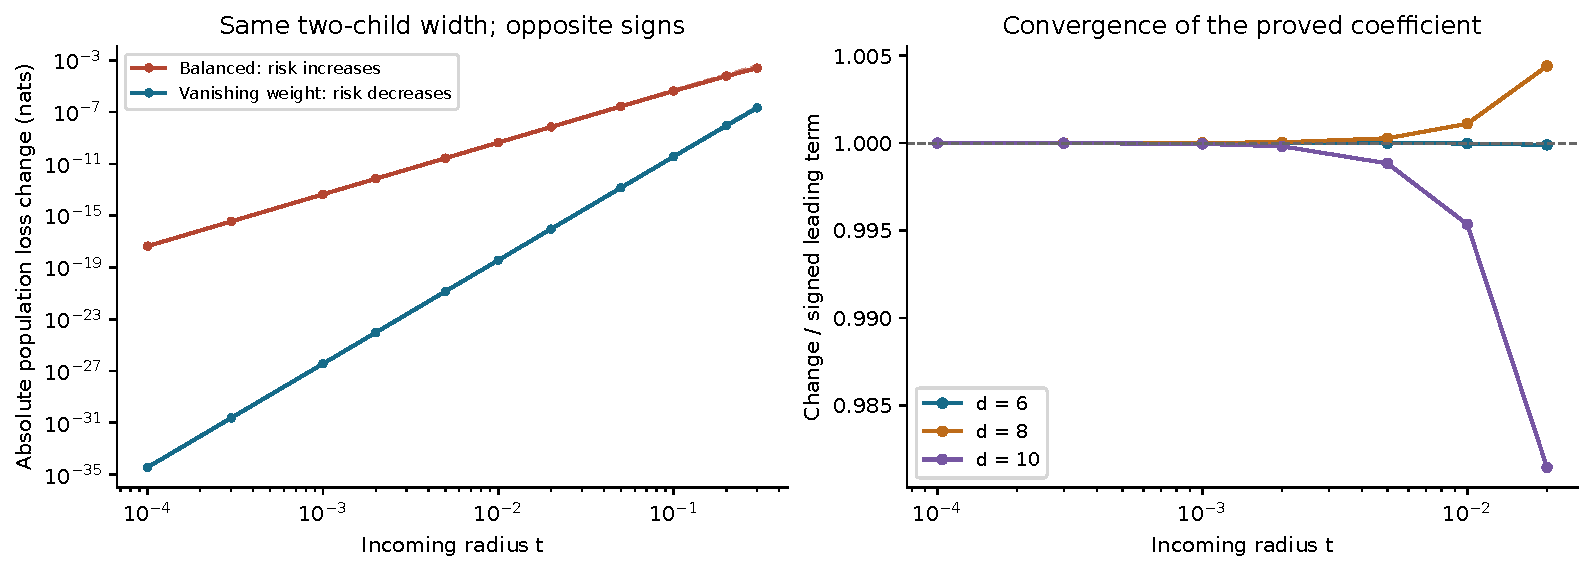
\includegraphics[width=\linewidth]{high_order_limits.pdf}
\caption{Exact population calculations, not training. Left: absolute loss
change for balanced positive splitting (increases) and the vanishing-proportion
path (decreases) at $d=6$. Curves use saved high-precision outputs; dashed
curves are proved leading terms. Right: the measured change divided by its
signed leading term for $d=6,8,10$. The right panel restricts to smaller radii
to show the asymptotic regime. Both operations use two children
and outgoing absolute sum one. The diminishing gain is shown explicitly.}
\label{fig:highorder}
\end{figure}

For $d=6,t=0.1$, balanced splitting changes risk by
$+4.2255\cdot10^{-6}$ nats; the vanishing proportion
$p=0.00286119$ changes it by $-3.5902\cdot10^{-11}$ nats.
At the same radius the latter gains for $d=8,10$ are approximately
$8.47\cdot10^{-16}$ and $3.68\cdot10^{-20}$ nats.
The task-information gap is about $0.04570$ nats in every case.
Strict descent therefore does not constitute a useful trained classifier.
The asymptotic gain is not uniform over radius: for $d=10,t=0.3$, the
vanishing-proportion formula actually increases risk by
$3.46\cdot10^{-12}$ nats, a saved finite-radius failure.
A coefficient three times the asymptotically minimizing $\kappa$ reverses
the small-radius improvement in the independent check, demonstrating that
merely making a child small is insufficient.

We also ran finite-observation tests of Proposition~\ref{prop:snr} for $d=6$.
For each of four radii and five sample sizes, 1,000 independent repetitions
estimate the raw score. Sampling uses multinomial counts of the exact iid
input--label categories; this is ordinary random sampling represented by
sufficient counts, with no importance weighting or population labels in
the estimate. A comparator receives the true parity feature and estimates
its label correlation on the same samples. That feature is privileged
structural information and is explicitly not an equally informed controller.

\begin{figure}[tb]
\centering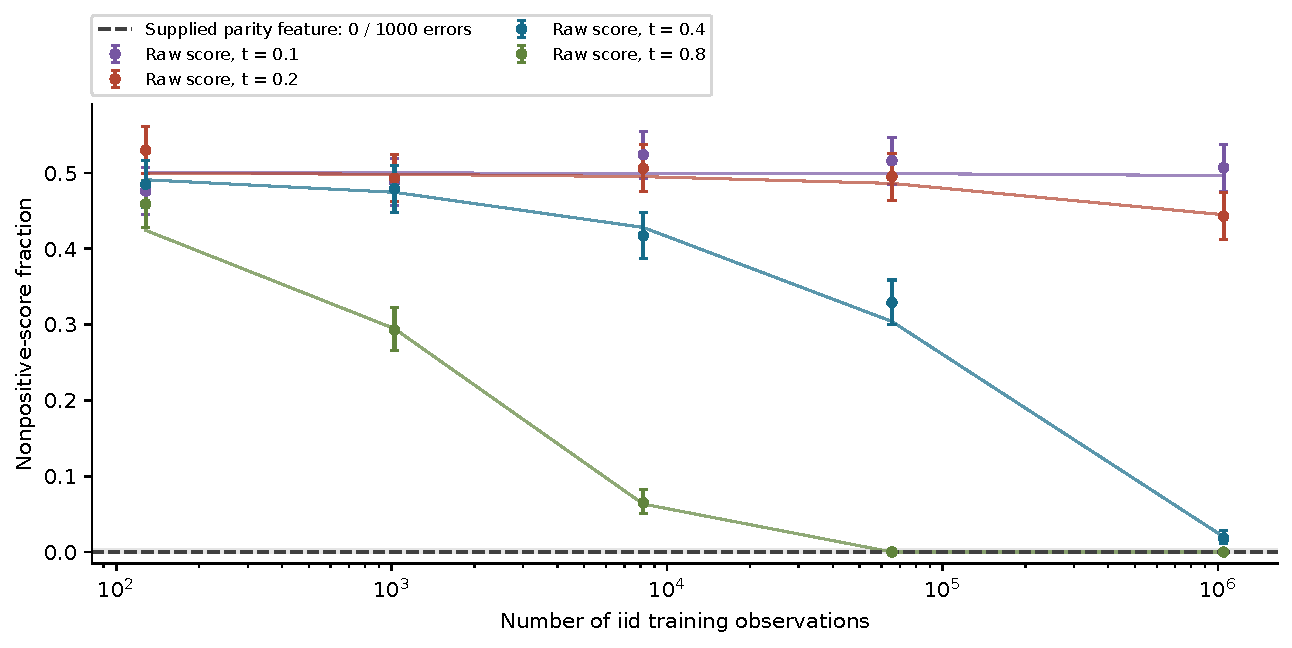
\includegraphics[width=.94\linewidth]{score_sampling.pdf}
\caption{Finite iid score estimation on the six-bit noisy-parity task.
Points show the fraction of nonpositive estimated scores across 1,000
repetitions; bars are pointwise 95\% Wilson binomial intervals. The population
score is positive. Curves are normal-approximation predictions using exact
population means and variances, not fitted error rates or guarantees.
The dashed reference uses a supplied true-parity feature and has zero
observed failures in these runs; its uncertainty remains nonzero.
No neural parameters are trained in this figure.}
\label{fig:sampling}
\end{figure}

At $t=0.1,n=1{,}048{,}576$, the raw score has the wrong or zero sign in
507 of 1,000 repetitions. Its unit-signal-to-noise sample proxy is
$1.3844\cdot10^{10}$ observations. At $t=0.4$ the same sample size has
18 failures and the proxy is $2.4928\cdot10^5$. The supplied parity feature
has no observed sign errors across the tested conditions. These measurements
show the cost of this raw score, not a minimax lower bound on learning
parity, nor a claim that a known feature is free to discover.

\section{Finite-sample neural growth: realized effects and failed extensions}
\label{sec:experiments}

The preceding statements concern population risks and prescribed operations.
We therefore conducted actual neural training experiments in which the controller
observes only sampled labels. These experiments test three different questions:
can sampled operational statistics recover the useful split direction; does that
initial advantage survive optimization; and can an empirical gate avoid
unnecessary growth? A separate exploration tests a conditional-information
operation score under ordinary random neural initialization. None of these
experiments identifies representation states with neurons.

\subsection{Parameterized system and controller information}

The trained predictor is
\[
 p_\theta(x)=\operatorname{sigmoid}\left(c+\sum_{j=1}^k
 a_j\tanh(b_j+w_j^\top x)\right).
\]
The trainable objects are actual hidden units with input weights $w_j$, biases
$b_j$, output coefficients $a_j$, and a common intercept $c$. A split duplicates
unit $j$, halves its output coefficient, and replaces its two input weights by
$w_j+\varepsilon v$ and $w_j-\varepsilon v$. All input weights, hidden biases,
output coefficients, and the intercept are subsequently trained without a tying
constraint. At $\varepsilon=0$ this operation preserves the predictor exactly;
for positive $\varepsilon$ it is a controlled perturbation, followed by a real
change in parameter count. Retraining may change predictions at every old input.
It need not create a nested discrete partition.

For the theory-linked experiment, the learned direction is the smallest
eigenvector of
\[
 \widehat S_j=\frac1n\sum_{i=1}^n
 [p_\theta(x_i)-y_i]a_j\tanh''(b_j+w_j^\top x_i)x_ix_i^\top.
\]
This is an operation-specific curvature statistic, not marginal activation
entropy. Its implementation observes input coordinates, residuals, and the
current parameters. It receives neither the population conditional label
probabilities nor a supplied signal direction. The random-direction control
uses a normalized standard Gaussian vector. A separately labelled population
curvature oracle computes $S_j$ from the complete known synthetic population;
it is a diagnostic and does not enter either learned controller. At the
constant start, an activation-only scalar statistic has no directional
information; the random control is the deliberately uninformative directional
comparison, rather than an invented entropy optimizer.

\subsection{The controlled bridge and its validity tests}

We use five regimes. The four-state regime is uniform on
$\{\pm e_1,\pm e_2\}$ with conditional label probabilities $0.65$ on the first
axis and $0.35$ on the second. The width-one initial parameters are
$w=0$, $b=0.5$, $a=1$, and $c=-\tanh(0.5)$, so the initial prediction is $1/2$.
The rotated regime is uniform on the sixteen points $\{\pm Qe_j:1\leq j\leq8\}$,
where each repetition draws a new orthogonal matrix by QR factorization of a
Gaussian matrix. Label probabilities are $0.65$ and $0.35$ on its first two
axes and $0.5$ on the remaining axes. Thus the controller must discover the
input geometry amid six irrelevant axes. The sample-pretrained regime uses
this rotated task but first trains the width-one model for 100 updates from
the special initialization. The random-start regime instead initializes all
width-one weights randomly and trains for 100 updates. The no-signal regime
uses the rotated inputs with every label probability equal to $0.5$.
These tests distinguish a deliberately designed stationary start from a
checkpoint obtained through ordinary sample training.

Each regime uses $n\in\{256,1024\}$ IID training examples and an independent
validation sample of the same size. A sample contains ordinary Bernoulli labels;
there is no importance sampling or enumerated-label training. The split uses
$\varepsilon=0.6$. Each branch receives either $T=30$ or $T=300$ full-batch Adam
updates with learning rate $0.02$, standard momentum coefficients $0.9,0.999$,
and numerical denominator constant $10^{-8}$. Optimizer moments are reset at
each branch, including the continuation control. The shared pre-split checkpoint
is identical for the spectral, random, and oracle branches. All parameters are
untied and trained after the split. The two budgets are separate runs, not
selected stopping times. For numerical stability, the code clips
predicted probabilities to $[10^{-9},1-10^{-9}]$ for evaluation; the
maximum absolute logit across all saved fitted bridge branches is 6.852,
well inside the clipping threshold of 20.723. Thus that clip does not
alter their reported population losses.

There are 64 independent repetitions per regime, sample size, and budget,
using seeds 27100 through 27163. This gives 1280 completed training configurations.
Shared random seeds make within-configuration method comparisons paired;
confidence intervals never treat the methods or input points as independent
replicates. We report Student-$t$ intervals across the 64 seed-level paired
risk differences. They are descriptive intervals for these synthetic regimes,
without a multiple-comparison claim. Risk evaluation integrates both the finite
input distribution and the conditional label law exactly. This exact evaluation
is distinct from the finite-sample learning that produced each network.

The autonomous variant fits both the grown model and a width-one continuation.
On the disjoint validation sample it computes their paired per-example log-loss
improvements $D_i$, accepting growth only if
$\overline D>1.96\,s_D/\sqrt n$. Otherwise it keeps the continuation.
This fixed normal-approximation rule is a heuristic gate, not a theorem-level
finite-sample confidence guarantee. Both spectral and random proposals use the
same rule and validation sample. The gate therefore does not silently borrow
population information, but it does pay for two fitted branches and additional
labelled validation data. Its comparison with an ungated continuation does not
by itself isolate the value of the spectral principle.

\subsection{Capacity, compute, data, and implementation controls}

A width-$k$ model in dimension $d$ has $k(d+2)+1$ trainable parameters. The bridge
therefore grows from $d+3$ to $2d+5$ parameters. Spectral and random growth have
identical final architecture, shared initialization, training data, update count,
and optimizer. Their additional controller costs differ: forming the spectral
matrix costs $O(nd^2)$ arithmetic and its eigendecomposition costs $O(d^3)$;
random direction generation costs $O(d)$. These overheads are explicitly
additional, although small in these low-dimensional experiments.

We also train fixed width-two networks from standard random initialization.
One comparison matches the number of optimization updates, including any
width-one pretraining. A second matches the approximate number of
parameter-example updates: after $P$ pretraining steps and $T$ growth steps,
the fixed model receives
\[
 T+\left\lfloor\frac{P(d+3)}{2d+5}\right\rfloor
\]
updates. This is an operation-count proxy, not a claim of identical measured
FLOPs, optimizer cost, or wall time. $P=0$ for the prescribed stationary starts
and $P=100$ for the two pretrained regimes. We do not call equal updates and
equal compute the same comparison. All methods use the same training examples;
only gated decisions consume the separate validation labels. Raw records retain
these resource formulas, controller costs, selected directions, split matrices,
immediate and post-training risks, validation events, prediction changes,
parameter displacements, and fitted network parameters.

The reported parameter counts describe individual predictors, not total live
process memory. A gate retains a continuation and a growth candidate, together
with optimizer state during fitting; its peak memory and branch-training cost
exceed the final predictor size. The implementation additionally fits every
comparison and oracle for measurement. Those research costs cannot be credited
as free online adaptation. The entire 1280-configuration bridge run took
85.53 seconds on the local CPU environment; this aggregate wall time is not a
per-method runtime comparison.

Independent implementation checks compare analytic gradients against central
finite differences (maximum absolute error $8.16\times10^{-11}$), verify exact
function preservation at zero split displacement, and compare the actual
small-displacement risk change with the derived quadratic term. At
$\varepsilon=10^{-4}$ their ratio is $1.000000199$. These checks support the
implementation; they do not replace the mathematical proofs.

\begin{table}[tb]
\centering\footnotesize\setlength{\tabcolsep}{4pt}
\caption{Actual finite-sample neural training at $n=1024$. Entries are exact population log loss after fitting; $\Delta$ is the paired spectral-minus-random mean with a 95\% Student-$t$ interval half-width across 64 independent seeds. $T$ is the post-growth update budget. Fixed width uses the approximate parameter-update budget described in the text. Lower is better.}
\label{tab:neural-results}
\begin{tabular}{@{}llrrrrr@{}}
\toprule
Regime & $T$ & Spectral & Random & Fixed 2 & Continue 1 & $\Delta\pm$ half-width\\
\midrule
Four states & 30 & 0.65606 & 0.66809 & 0.68782 & 0.69323 & $-0.012033 \pm 0.003104$ \\
Four states & 300 & 0.64928 & 0.64928 & 0.65256 & 0.68002 & $-0.000002 \pm 0.000003$ \\
Rotated 8D & 30 & 0.69175 & 0.69458 & 0.69526 & 0.69744 & $-0.002827 \pm 0.000588$ \\
Rotated 8D & 300 & 0.68955 & 0.68971 & 0.69159 & 0.69488 & $-0.000162 \pm 0.000251$ \\
Random start & 30 & 0.69473 & 0.69450 & 0.69352 & 0.69450 & $+0.000236 \pm 0.000180$ \\
Random start & 300 & 0.69373 & 0.69371 & 0.69124 & 0.69421 & $+0.000019 \pm 0.000609$ \\
No signal & 30 & 0.69866 & 0.69797 & 0.69640 & 0.69770 & $+0.000691 \pm 0.000179$ \\
No signal & 300 & 0.70064 & 0.70068 & 0.70008 & 0.69805 & $-0.000046 \pm 0.000064$ \\
\bottomrule
\end{tabular}
\end{table}


\begin{figure}[tb]
 \centering
 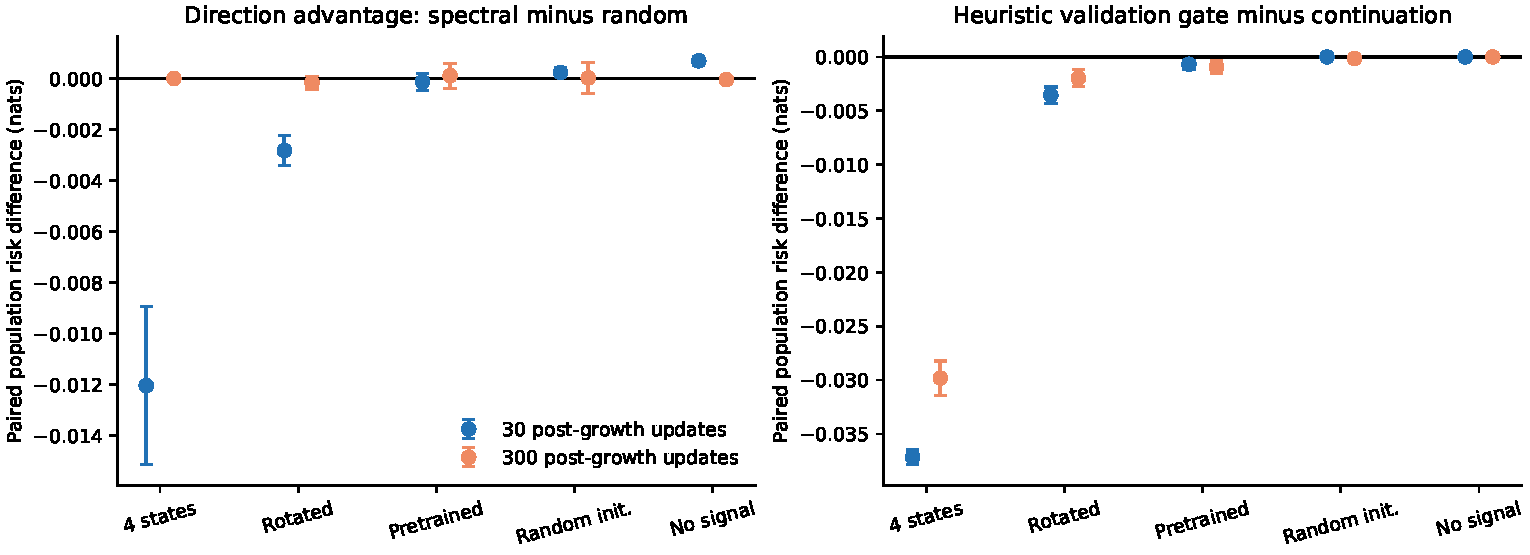
\includegraphics[width=\textwidth]{../figures/learning_curvature_differences.pdf}
 \caption{Measured neural training results at $n=1024$. Left: spectral minus
 random split risk at identical architecture and training budgets. Right: the
 heuristic validation-gated spectral model minus width-one continuation; this
 latter comparison additionally uses validation labels and branch-training
 compute. Points average 64 paired repetitions; bars are 95\% Student-$t$
 intervals. Every risk is evaluated exactly on the finite population after
 fitting from IID labelled samples. Negative values favor the spectral or
 gated method.}
 \label{fig:bridge-differences}
\end{figure}

\subsection{What the bridge established, and where it failed}

At the prescribed four-state start the learned spectral direction selects the
correct axis in all 64 repetitions at both sample sizes. Its immediate
population loss reduction is $0.00759820$ nats; random directions have negative
mean reductions, i.e. they initially increase the loss. At $n=1024$ and 30
updates, spectral growth has mean risk $0.656061$, compared with $0.668094$ for
random growth. Because those branches share the same capacity, data, training
budget, and initial checkpoint, this is evidence for the operational direction
choice in the designed regime, subject to its extra matrix-estimation cost.
After 300 updates their risks are $0.649278$ and $0.649280$; the directional
advantage has essentially disappeared. Thus the local geometric advantage is
not a persistent representational advantage when later optimization can
reorganize both models.

On the rotated task, the spectral proposal immediately improves population
loss in 44 of 64 repetitions at $n=256$ and 61 of 64 at $n=1024$. Its immediate
mean gain rises from $0.001245$ to $0.001795$ nats, compared with $0.001900$ for
the population curvature oracle. At $n=1024$ its 30-update advantage over random
splitting is $0.002827$ nats; it shrinks to $0.000162$ after 300 updates.
At $n=256$, longer retraining instead overfits: spectral population risk grows
from $0.709556$ after 30 updates to $0.722064$ after 300, both above the
constant-predictor risk $\log 2$. This is not hidden by reporting only ratios or
training accuracy.

The sample-pretrained and random-start tests are essential limitations.
After ordinary width-one sample training, the selected spectral direction is
no longer reliably aligned with the designed signal. In the random-start
regime at $n=1024$, its 30-update risk is slightly higher than random growth
($0.694734$ versus $0.694498$). At 300 updates there is no resolved difference.
The experiment therefore does not establish a generally useful growth rule at
arbitrary trained checkpoints. Moreover, finite-sample training can move along
initially neutral parameter directions and escape the particular population
local minimum: width-one continuation is not required to remain constant.
The observed continuation improvements do not contradict a local population
statement at a specified parameter point.

Every forced spectral split in the no-signal task increases the immediate
population loss. At $n=1024$ the validation gate accepts zero of 64 spectral
proposals at both budgets; at $n=256$ it accepts one of 64 at each budget.
On the rotated $n=256$, 300-update condition it rejects all 64 proposals,
preventing selection of the heavily overfit grown networks. Rejection is
relative to a fitted continuation, which may itself overfit; the gate does not
recover the unknown Bayes predictor or prove universally safe adaptation.
These are empirical gate diagnostics, not an automatic conversion of the
curvature theorem into a finite-sample acceptance guarantee.

\subsection{Independent random-initialization information-score probe}
\label{sec:information-probe}

Before choosing the theory-linked experiment, an independent investigation
implemented actual width-two to width-three growth on continuous Gaussian
inputs. It initially used the conditional label information of the
\emph{antisymmetric child-activation contrast}
$\tanh(a+\delta u)-\tanh(a-\delta u)$, where
$a=b_j+w_j^\top x$ and $u=v^\top x$.
Independent adversarial review identified a material limitation: this feature
contrast is not the symmetric predictor deformation caused by the prescribed
initial split. Its negative result cannot establish failure of an
operation-aligned information score. We retain all original runs and add a
fresh-seed ablation with the exact initial logit deformation
\[
 Z_v(x)=a_j\left\{\frac{\tanh(a+\delta u)+\tanh(a-\delta u)}2-\tanh(a)\right\}.
\]
The corrected feature definition was fixed before drawing its new seeds.

Each candidate is scored by the plug-in conditional mutual information between
its three-bin feature and the binary target, conditional on a three-quantile-bin
current prediction. The aligned feature uses three empirical quantile bins.
The original antisymmetric feature instead uses the fixed thresholds
$-0.08,0.08$; its marginal entropy is retained as a separate baseline. Thus
``entropy'' here refers to that specified three-state activation-contrast
histogram, not differential entropy. The conditioning variable is a lossy
quantization of the current prediction, not the full neural representation.
Consequently neither score is automatically the recoverable predictive
information of the full model, and neither provides a Bayes-refitting guarantee
for the trained network.

For each run, 512 examples train the network, 512 disjoint labelled examples
score candidate operations, and 8192 independent inputs evaluate it using the
known teacher label probabilities. This evaluation integrates the conditional
Bernoulli label law exactly but only Monte Carlo averages the continuous input
distribution; it is not an exact population calculation. Population probabilities
are never passed to learned selectors. The deliberately optimistic evaluation
oracle chooses the candidate with minimum loss on those same 8192 evaluation
inputs, and is labelled as an evaluation oracle rather than an implementable
controller or an exact population optimizer.

All three tasks use $X\sim N(0,I_3)$ and
$P(Y=1\mid X)=0.05+0.90\operatorname{sigmoid}(g(X))$.
The linear-null task has $g(x)=2x_1$. The localized task has
$g(x)=1.5x_1+4\tanh(2x_2+1)\tanh(2x_3-1)$.
The teacher task uses four tanh units with fixed weights, biases, and output
coefficients specified exactly in the released code. Width-two students start
randomly and receive 300 full-batch Adam updates with learning rate $0.025$.
Each of the two units has four independently drawn Gaussian split directions,
normalized to unit length, for eight candidate operations. The perturbation
scale is $\delta=0.25$ and each candidate then receives 150 updates of all
parameters. Random choice, the two information scores, and marginal entropy
select among the same candidates before retraining. A separately labelled
trained-validation control trains all eight candidates and selects by score-set
log loss. It has an eightfold candidate-fitting cost; that benefit cannot be
credited to a cheap information score. Width-two continuation and fixed
width-three controls receive the corresponding prescribed update budgets.
Information scoring uses 512 additional labelled score examples; random
selection does not use those labels, and the entropy proxy uses only score
inputs. Therefore any positive comparison with random selection would also
have to account for this extra supervised information. Here no resolved aligned
CMI advantage survives even with that access. The fixed-width approximate
compute comparator scales the width-two pretraining budget by $2/3$, explicitly a leading-width proxy rather than exact
parameter/FLOP matching.

The original four-seed pilot used 250 pretraining updates and is preserved;
subsequent exploratory and aligned runs use 300. Thus the pilot-to-expanded
comparison does not change only the repetition count. The 32-seed exploratory
run is also preserved, with seeds $17000,\ldots,17031$. The aligned ablation uses 32 new seeds
$41000,\ldots,41031$ after the audit-triggered definition change. No fresh evaluation
result was used to tune that feature definition, the bin count, the optimizer,
or the candidate perturbation. It remains a small synthetic mechanism study,
not a broad benchmark or a universal rejection of information-guided growth.

For complete specification, the teacher function is
$g(x)=\tanh(x^\top W+\beta^\top)\alpha$ with
\[
 W=\begin{pmatrix}
 1.8&-1.4&0.4&1.2\\
 0.4&1.8&-1.7&0.8\\
 -1.5&0.3&1.3&-1.2
 \end{pmatrix},\qquad
 \beta=(0.4,-0.5,0.2,1)^\top,\qquad
 \alpha=(2,-2,2,-1.5)^\top.
\]
Standard random initialization in both studies uses independent input weights
$N(0,0.8^2)$, hidden biases $N(0,0.1^2)$, output coefficients
$N(0,0.5^2)$, and intercept zero.

\begin{table}[tb]
\centering\footnotesize\setlength{\tabcolsep}{5pt}
\caption{Fresh-seed operation-aligned information-score ablation. Risks integrate the teacher label probability on 8192 held-out Gaussian inputs, and are averaged across 32 seeds. The last column gives aligned-CMI minus random-growth risk with a paired 95\% Student-$t$ interval half-width. Fixed width 3 uses the leading-width compute proxy; its initialization differs from the grown model.}
\label{tab:aligned-probe}
\begin{tabular}{@{}lrrrrr@{}}
\toprule
Task & Aligned CMI & Random & Entropy & Fixed 3 & Difference $\pm$ half-width\\
\midrule
teacher & 0.40350 & 0.40250 & 0.40364 & 0.40093 & $+0.00100 \pm 0.00159$ \\
localized & 0.51857 & 0.51594 & 0.49348 & 0.48874 & $+0.00263 \pm 0.00991$ \\
linear null & 0.53534 & 0.53601 & 0.53724 & 0.53359 & $-0.00067 \pm 0.00235$ \\
\bottomrule
\end{tabular}
\end{table}


\begin{figure}[tb]
 \centering
 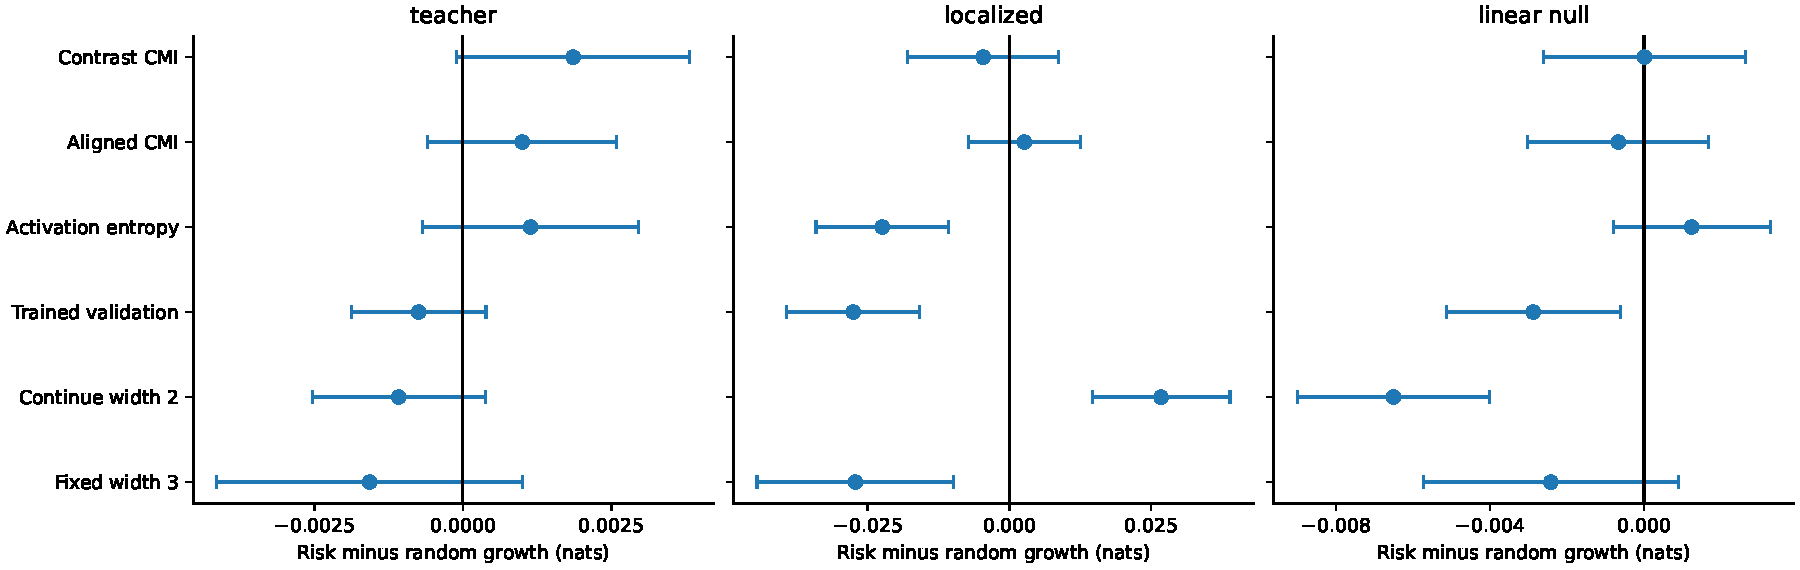
\includegraphics[width=\textwidth]{../figures/learning_information_aligned.pdf}
 \caption{Fresh-seed information-score ablation: paired risk differences from
 random growth over 32 independent repetitions, with 95\% Student-$t$ intervals.
 Aligned CMI uses the exact initial symmetric split logit deformation; contrast
 CMI uses the original antisymmetric activation contrast. Trained validation
 fits all eight candidates; fixed width 3 has a distinct initialization and a
 leading-width compute proxy. Risks average the true conditional label loss
 over 8192 held-out Gaussian inputs, not an exactly enumerated population.
 This plot is generated solely from saved experimental outputs.}
 \label{fig:aligned-information}
\end{figure}

The aligned score does not show a resolved advantage over random growth in
any of these three tests. Its paired mean differences are
$+0.000999\pm0.001588$ nats on the teacher task,
$+0.002634\pm0.009912$ on the localized task, and
$-0.000666\pm0.002350$ on the linear-null task, where each uncertainty is a
95\% Student-$t$ interval half-width across the 32 fresh seeds.
The localized task offers clear scope for improvement from additional capacity,
but the aligned information score does not identify the most useful operation:
its mean risk is $0.518572$, compared with $0.493478$ for the specified entropy
proxy and $0.488745$ for the fixed-width approximate-compute control.
The entropy proxy has a paired advantage over random growth of
$0.022459\pm0.011681$ nats on this task, whose interval excludes zero; this
positive measured finding is retained alongside the information-score nulls.
This observation does not make marginal activation entropy a valid invariant
principle. It shows that, in this experiment, the proposed label-information
proxy failed even to outperform a simple competing score.

On the linear-null task, continuing width two achieves mean risk $0.529499$,
below the aligned-growth risk $0.535339$. Information-score selection in this
study was forced to grow and therefore did not itself solve the decision of
whether to grow. Trained validation often improves candidate selection, but it
pays to fit all candidates and is not evidence for a cheap information-based
controller. The original 32-seed antisymmetric-proxy run is also preserved:
its apparent four-seed localized-task benefit did not become a resolved
conditional-information advantage after expansion. The audit-triggered aligned
ablation prevents that initially flawed proxy from carrying the conclusion.

The supported advance is consequently narrow and explicit. Input--residual
geometry can identify a beneficial real neuronal operation from finite samples
at a constructed stationary checkpoint, whereas unit-local scalar observables
cannot identify its direction. Equal-capacity neural training verifies that
this matters under a short optimization budget. Longer training, ordinary
pretraining, irrelevant inputs, and no-signal tasks expose its limitations.
The information-score experiments further show that defining and estimating a
conditional label-information quantity does not by itself supply an effective
neural structural controller. These findings establish a testable bridge and
its failure boundaries, not a general autonomous architecture-learning method.

All raw runs, failed or unfavorable conditions, seed ranges, learned matrices,
model parameters, resource proxies, and rerunnable figure scripts are included.
The main neural studies use only the existing local NumPy/SciPy environment;
no GPU, cloud resource, paid API, external dataset, or system-wide installation
was used. The experiments contain one structural decision per run and do not
establish the behavior of repeated, lifelong growth.


\section{What this advances, and what remains unsupported}
\label{sec:limits}
Relative to Phase I, this work replaces a purely finite-representation
obstruction with explicit neural parameters, finite observations, and
actual learning. It does not identify neural width with the number of
representation states. The observation theorem explains why a scalar
information content or an activation summary can fail to determine a useful
operation even when the relevant information is present in the input.
The sample theorem gives a realizable context-based decision with a
matching necessary sample order in that restricted problem. The singular
positive split theorem shows that width alone also misses a resource:
how outgoing proportions and incoming movement approach the structural
change, even without negative weights or extra children.

The trainable step achieved is modest but concrete. A controller computes
an empirical statistic from a unit's input and residual, selects a real
neural duplication direction, trains both resulting hidden units, and can
accept or reject growth using a disjoint holdout set. The evidence establishes
its short-budget benefit at a constructed stationary point and measures
where that benefit disappears. It does not establish that activation entropy,
conditional information, or split curvature is generally the right trigger
for autonomous structure adaptation. One-event growth and rejection are
implemented; a stable repeated lifetime controller is not.

Several boundaries carry the conclusions. The activation-only theorem is
about a passive pre-operation observation channel; ordinary subsequent
training or active input-dependent probing can break indistinguishability.
The high-order proof keeps an intercept and a particular operation family
fixed, and selects its direction and coefficient with population knowledge.
It is not a guarantee that SGD discovers a vanishing-weight path. Its
population gains can be many orders smaller than sampling error or numerical
precision. The neural experiments are small synthetic tanh classifiers,
not broad deep-learning benchmarks, biological neuron models, or tests of
nonstationary continual learning. Fixed-width baselines often match or
outperform the adaptive alternatives. Parameter-update proxies do not
measure hardware FLOPs, memory, or wall-clock efficiency of a deployable
controller. Holdout gating consumes another fitted branch and extra data;
its normal approximation is not a theorem-level certificate.

The nearest-source review substantially limits the novelty claim: known
curvature growth and known boundary escape provide the foundation. The new
claims are the exact observation/task witness with quantitative evidence
requirements and the constrained positive-weight joint-limit separation,
together with openly adverse implementation evidence. Their equivalence
to a broader existing formulation remains a question for external review.
The project supplies complete proofs, independent checks and raw results,
but does not claim external peer review or publication readiness.

\section{Reproducibility and research record}
All Phase II materials are under \texttt{phase2/}. The top-level Phase I
manuscript and outputs remain unchanged. \texttt{README.md} gives exact
commands; \texttt{code/reproduce.py} regenerates the performed computations,
figures and paper. Raw outputs distinguish exploratory pilots, the expanded
probe, the new operation-aligned evaluation, the curvature bridge, population
calculations and sample-only tests. Saved seeds and deterministic generators
reconstruct all data. The neural bridge saves event directions, matrices,
acceptance decisions, post-operation risks and parameters. It does not
pretend to log every optimizer iterate.

The runtime is local macOS arm64, Python 3.12.14, NumPy 2.3.5,
SciPy 1.18.1, mpmath 1.3.0 and Matplotlib 3.11.2, with eight reported
logical CPUs. NumPy CPU training avoids a missing PyTorch dependency.
No paid API, remote GPU, publishing service, private data upload, or
system-wide installation was used. LaTeX/Poppler compile and render the
companion PDF. A concise status file and contribution/evidence ledger
record completed work, corrections, objections and remaining gaps.

Independent numerical implementations cross-check the proof calculations and
learning routines. The high-order direction was revised after counterexample
search, and the information-probe mismatch was corrected by an additional
operation-aligned evaluation with new seeds. These historical checks do not
constitute external peer review.

\bibliographystyle{plainnat}
\bibliography{references}
\end{document}
